\subsection{NVAR Results}
\label{subsec:nvar-results}


\subsubsection{Temporal Subsampling}


\begin{figure}
    \centering
    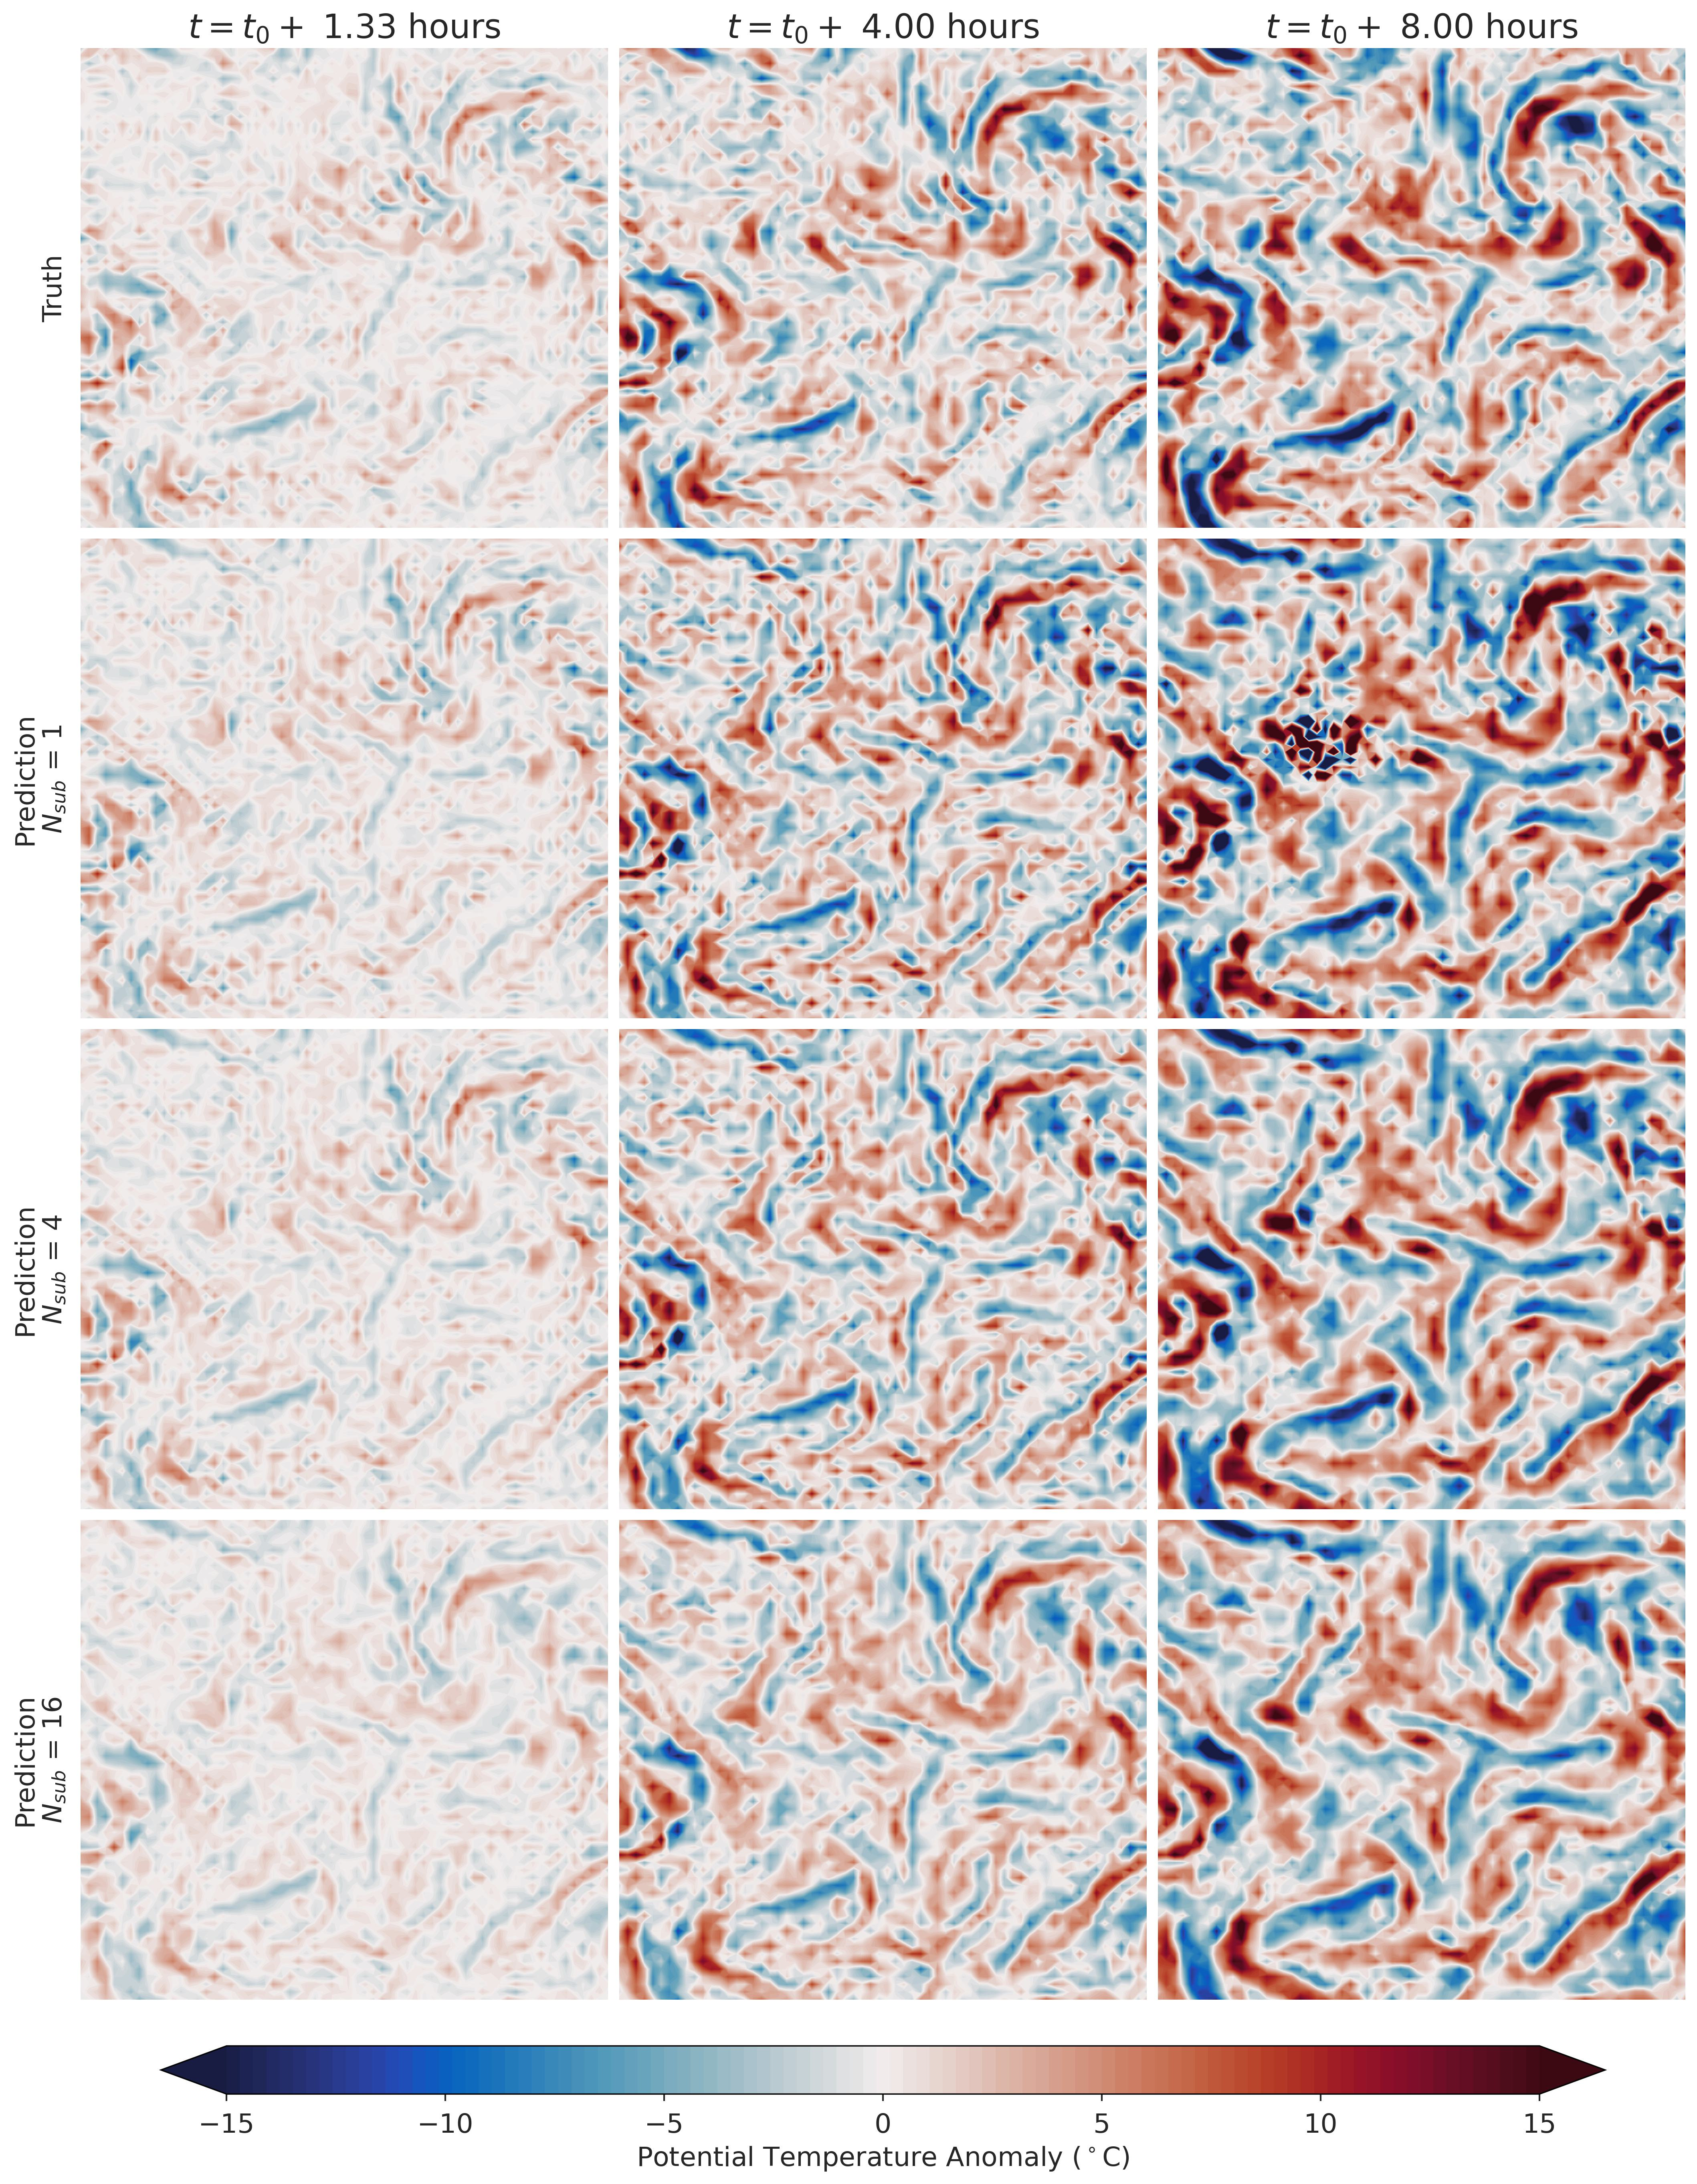
\includegraphics[width=\textwidth]{../figures/nvar_big_plot.jpg}
    \caption{One sample NVAR prediction from the test dataset for $\nsub =
        1,4,16$, shown in the second, third, and fourth rows.
        The corresponding truth is shown in the top row.
        In order to emphasize the changing features in the plot, each panel
        shows the difference between the state after 1.33, 4, and 8 hours with
        the initial conditions ($t_0$), corresponding to the left, middle, and
        right columns.
        Here $\maxlag=1$.
    }
    \label{fig:nvar_qualitative}
\end{figure}

% Describe the big plot
% diff btwn t0, Nlag=1, one sample from test dataset
\cref{fig:nvar_qualitative} shows a qualitative comparison of NVAR predictions
as a function of $\nsub$, i.e., how frequently the training data are sampled and
the model makes predictions.
Each panel shows the difference between a given timestep and the initial
conditions in order to emphasize the features that change over an 8~hour window.
The top row shows the truth, while subsequent rows show the evolution of NVAR
predictions for $\nsub=1,4,16$.
For this figure, we set $\nlag=1$, and note that the normalized root-mean-square
error (NRMSE) and Anomaly Correlation
Coefficient (ACC) corresponding to this configuration are shown in \red{FIG X},
indicating prediction skill across 50~samples in the test dataset.

% Describe qualitatively what happens as we subsample the data further
% At Nsub=1, unstable, some smoothness especially at longer times but less so at
% short times
% As Nsub increases, stable, but "more smooth" at small scales even at shorter
% prediction windows
At the model timestep ($\Delta \tau = \Delta t = 5$~min; $\nsub=1$), the NVAR predictions are
qualitatively similar to the truth for relatively short forecast windows.
That is, the NRMSE is near 0, and, visually speaking,
many of the fronts and dipoles that exist in the truth are also evident
in the predictions.
However, at longer forecast windows the predictions are unstable: NRMSE spikes
rapidly after about 4~hours and in \cref{fig:nvar_qualitative} instabilities are
present after 8~hours.

%Additionally, as the forecast develops, the prediction becomes somewhat smoother
%than the truth, which is evident as many small scale features are connected in
%the prediction.
As the temporal resolution of the data is reduced, i.e., as $\nsub$ increases,
the predictions are generally stable for a longer period of time.
\red{FIG X} shows that for $\nsub=4$, predictions are stable for roughly
6~hours, and for $\nsub=16$ no predictions generate instabilities over the
12~hour window.
However, this stability comes with a cost: as the temporal resolution is
reduced, the model's representation of small scale features diminishes as these
features become more blurry or smooth.
This blurring effect is apparent in \cref{fig:nvar_qualitative}, where at each
timestep (column), the prediction is progressively more blurry at larger values
of $\nsub$.
At $\nsub=16$ ($\Delta \tau = $1.33~hrs), the smoothing effect is
evident even after a single timestep (i.e., the first column in
\cref{fig:nvar_qualitative}),
as many small scale features are broader than the truth and fronts generally
exhibit lower amplitudes.

\begin{figure}
    \centering
    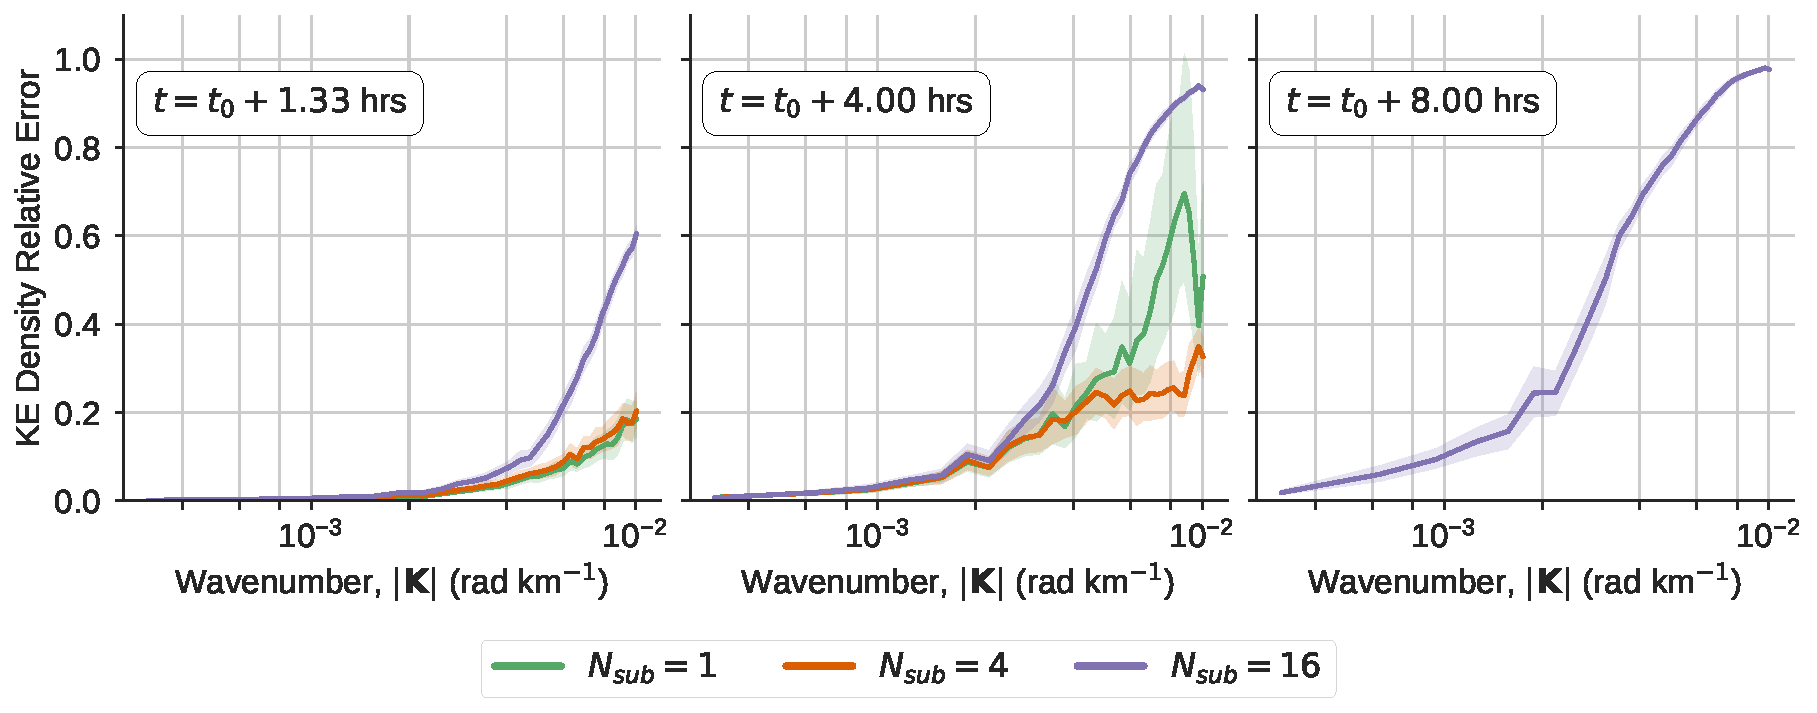
\includegraphics[width=\textwidth]{../figures/nvar_ke_relerr.pdf}
    \caption{NVAR Spectra}
    \label{fig:nvar_spectra}
\end{figure}

\begin{figure}
    \centering
    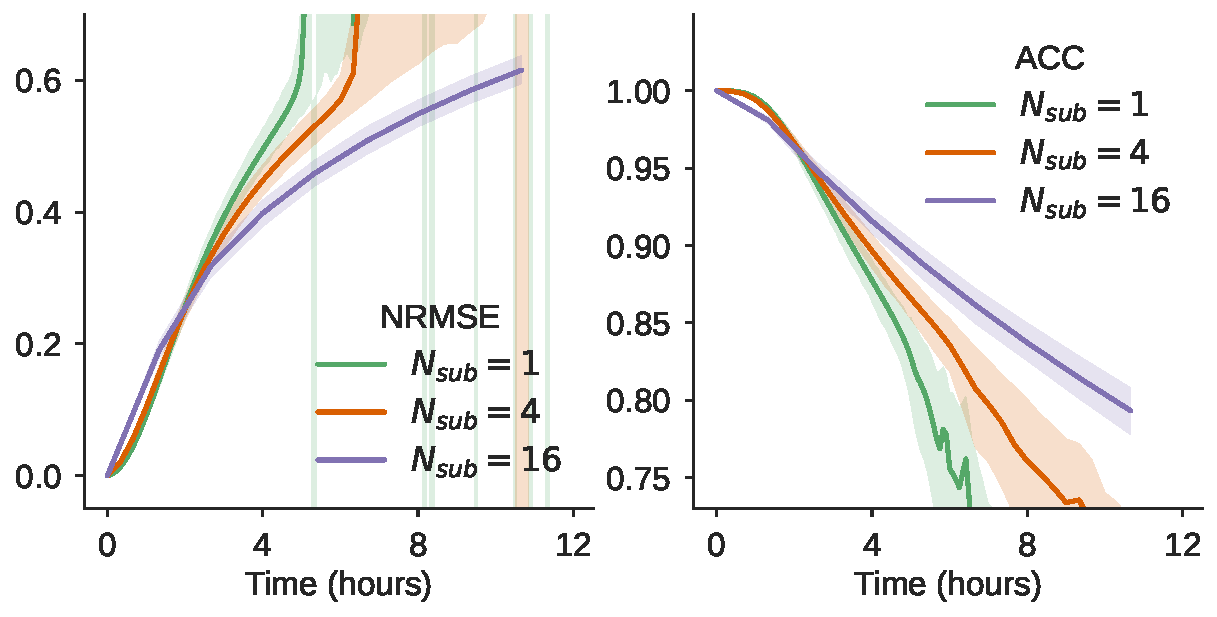
\includegraphics[width=\textwidth]{../figures/nvar_rmse_and_acc.pdf}
    \caption{NRMSE and ACC}
    \label{fig:nvar_nrmse_and_acc}
\end{figure}

% To show a quantitative discussion, consider the relative error in the KE density
% First column only: colors show error at different time stamps, spread
% indicates error over 50 samples in test dataset,
% In all plots, error is largest at the small spatial scales, corresponding to
% larger wavenumbers
% Note that not all of the Nsub=1,4 sims are stable, so the relative error is
% unacceptably large for t0+8 hrs, well beyond what is shown...
This smoothing behavior is captured quantitatively in \cref{fig:nvar_spectra},
which shows the relative error in terms of the kinetic energy density spectral
coefficients as a function of forecast time (panels) and $\nsub$ (colors).
The solid lines indicate average error and the shading indicates a spread of one
standard deviation, computed based on 50~samples predictions each initialized
from different initial conditions in the test dataset.
Generally speaking, error is largest in all cases at smaller spatial scales,
which corresponds to the higher wavenumbers.
%Note also that not all of the predictions produced with $\nsub=\{1,4\}$ are
%stable, so the relative error is \red{unacceptably large} after 8~hours, and
%therefore not shown.

% Nsub=1,4 produce nearly identical errors at small scales for short lead times,
% Nsub 1 generates instabilities in many simulations early on, and so error is
% large
% by subsampling the data more dramatically, Nsub=16, we see the error in the
% small scales grows considerably (by at least 40%).
At short lead times, the relative error is smallest and nearly
identical for the high frequency simulations: $\nsub=\{1,4\}$.
However, as discussed above,
these predictions generate instabilities rapidly, and so the relative error is
greater than one by 8~hours.
By increasing the subsampling factor to $\nsub=16$, the simulations are stable
and relative error is less than or equal to one.
However, at all timesteps shown the relative error 2-3 times larger for wavenumbers
$> 4\cdot10^{-3}$~rad~km$^{-1}$.
This error at higher wavenumbers corresponds to the qualitatively smooth
prediction shown in \cref{fig:nvar_qualitative}, as the small spatial scale
features are simply not resolved.


\subsubsection{Prediction Skill as a Function of Memory}

% A key feature of RNNs and autoregressive models is memory
% NVAR gives us the opportunity to explore this explicitly.
A key feature of RNNs and autoregressive models is that they retain memory of
previous system states.
We explore the effect of adding memory within the NVAR architecture explicitly
by increasing $\nlag$, the largest number of lagged states used to create the
feature vector.
We summarize this behavior in \red{FIG NRMSE}, which shows the NRMSE as a
function of $\nlag$ (colors) for each
subsampling factor $\nsub = \{1, 4, 16\}$ (panels).
Generally speaking, adding memory (increasing $\nlag$) shows a similar behavior as increasing the
temporal resolution (decreasing $\nsub$): short term prediction skill improves,
while long term skill is diminished.

\begin{figure}
    \centering
    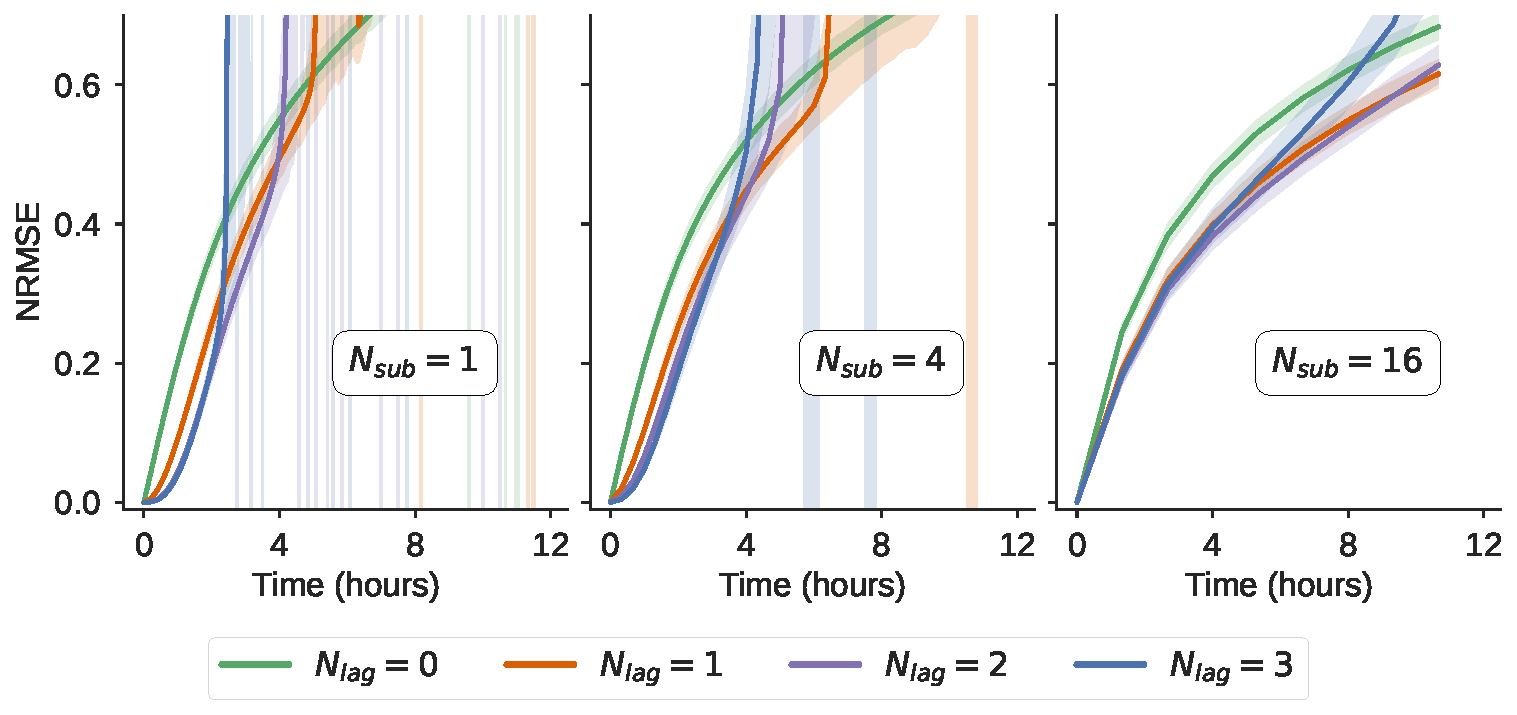
\includegraphics[width=\textwidth]{../figures/nvar_nrmse_vs_memory.pdf}
    \caption{NRMSE vs lag}
    \label{fig:nvar_nrmse_vs_lag}
\end{figure}

We suspect that increasing memory reduces long term prediction skill for two
reasons.
First, more time separation means more nonlinearity in its representation.
Secondly, error is more readily propagated from the small scales to the larger
scales because we retain more memory of previous errors.
This is shown in Fig X,
which shows the relative error in terms of kinetic energy density spectral coefficients for $\nsub=16$ and
$\nlag=\{0, 1,2,\text{ and }3\}$, respectively.
For about the first 4~hours, prediction skill is improved at all spatial scales.
However, beyond this point
NRMSE grows rapidly, the improvement at
small scales ($|\mathbf{K}|>2\cdot10^{-3}$~rad~km$^{-1}$) is more muted,
and error increases at the large scales.

\begin{figure}
    \centering
    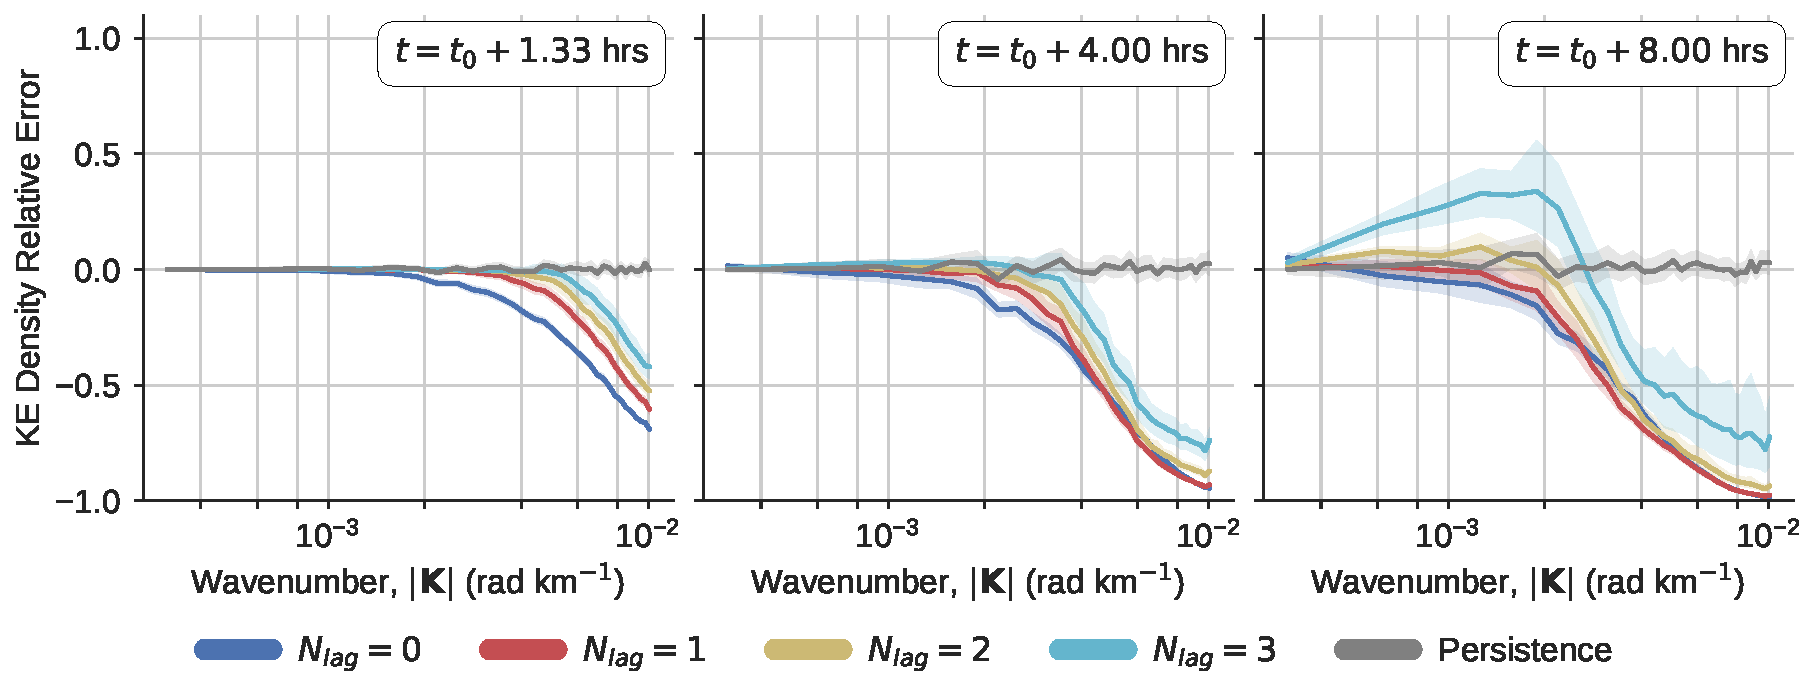
\includegraphics[width=\textwidth]{../figures/nvar_ke_relerr_vs_lag.pdf}
    \caption{KE Error vs lag}
    \label{fig:nvar_ke_vs_lag}
\end{figure}

\begin{figure}
    \centering
    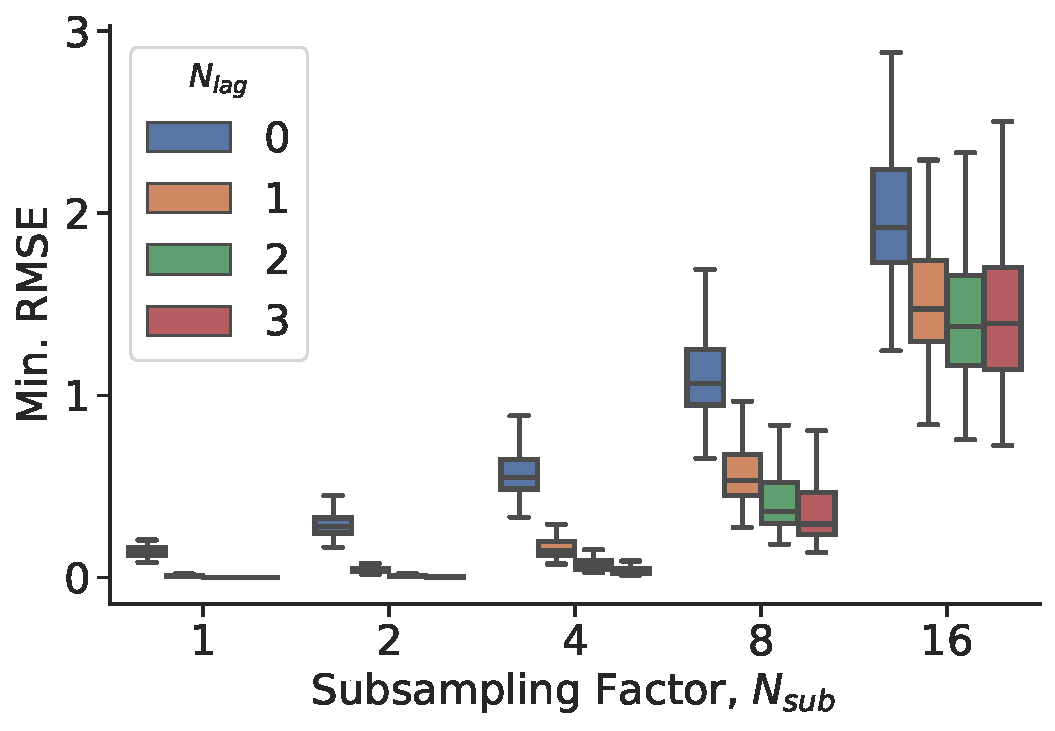
\includegraphics[width=.5\textwidth]{../figures/nvar-mrmse-vs-lag-050samples.pdf}
    \caption{Minimum RMSE}
    \label{fig:nvar_min_rmse}
\end{figure}

The behavior discussed here is summarized by the boxplots in
\cref{fig:nvar_min_rmse}, which shows the minimum RMSE achieved by NVAR for a
given $\nsub$ (x-axis) and $\nlag$ (color).
The best prediction skill, which as we noted is achieved within the first
1-2~hours of the forecast, is best for smaller $\nsub$.
Increasing $\nlag$ can improve this prediction skill to make up for subsampled
data, albeit with dimishing returns.
Additionally, for $\nsub$ large enough
(here $>4$), the gains in ``best possible'' skill do not approach what can be
achieved with $\nsub\le 4$, presumably due to the fact that small scale features
cannot be resolved when enough temporal information is skipped.
